\documentclass{ximera}

\outcome{Use limits to find the slope of the tangent line at a point.}
\outcome{Understand the definition of the derivative at a point.}
\outcome{Compute the derivative of a function at a point.}
\outcome{Estimate the slope of the tangent line graphically.}
\outcome{Write the equation of the tangent line to a graph at a given point.}
\outcome{Recognize and distinguish between secant and tangent lines.}
\outcome{Recognize different notation for the derivative.}
\outcome{Recognize the the tangent line as a local approximation for a
  differentiable function.}

%\usepackage{todonotes}

\newcommand{\todo}{}

\usepackage{tkz-euclide}
\tikzset{>=stealth} %% cool arrow head
\tikzset{shorten <>/.style={ shorten >=#1, shorten <=#1 } } %% allows shorter vectors

\usepackage{tkz-tab}  %% sign charts
\usetikzlibrary{decorations.pathreplacing} 

\usetikzlibrary{backgrounds} %% for boxes around graphs
\usetikzlibrary{shapes,positioning}  %% Clouds and stars
\usetikzlibrary{matrix} %% for matrix
\usepgfplotslibrary{polar} %% for polar plots
\usetkzobj{all}
\usepackage[makeroom]{cancel} %% for strike outs
%\usepackage{mathtools} %% for pretty underbrace % Breaks Ximera
\usepackage{multicol}

\usepackage{polynom}



\usepackage[many]{tcolorbox}  %% for titled boxes
\newtcolorbox{xbox}[1]{%
    tikznode boxed title,
    enhanced,
    arc=0mm,
    interior style={white},
    attach boxed title to top center= {yshift=-\tcboxedtitleheight/2},
    fonttitle=\bfseries,
    colbacktitle=white,coltitle=black,
    boxed title style={size=normal,colframe=white,boxrule=0pt},
    title={#1}}


\usepackage{array}
\setlength{\extrarowheight}{+.1cm}   
\newdimen\digitwidth
\settowidth\digitwidth{9}
\def\divrule#1#2{
\noalign{\moveright#1\digitwidth
\vbox{\hrule width#2\digitwidth}}}





\newcommand{\RR}{\mathbb R}
\newcommand{\R}{\mathbb R}
\newcommand{\N}{\mathbb N}
\newcommand{\Z}{\mathbb Z}

%\renewcommand{\d}{\,d\!}
\renewcommand{\d}{\mathop{}\!d}
\newcommand{\dd}[2][]{\frac{\d #1}{\d #2}}
\newcommand{\pp}[2][]{\frac{\partial #1}{\partial #2}}
\renewcommand{\l}{\ell}
\newcommand{\ddx}{\frac{d}{\d x}}
\newcommand{\ddt}{\frac{d}{\d t}}

\newcommand{\zeroOverZero}{\ensuremath{\boldsymbol{\tfrac{0}{0}}}}
\newcommand{\inftyOverInfty}{\ensuremath{\boldsymbol{\tfrac{\infty}{\infty}}}}
\newcommand{\zeroOverInfty}{\ensuremath{\boldsymbol{\tfrac{0}{\infty}}}}
\newcommand{\zeroTimesInfty}{\ensuremath{\small\boldsymbol{0\cdot \infty}}}
\newcommand{\inftyMinusInfty}{\ensuremath{\small\boldsymbol{\infty - \infty}}}
\newcommand{\oneToInfty}{\ensuremath{\boldsymbol{1^\infty}}}
\newcommand{\zeroToZero}{\ensuremath{\boldsymbol{0^0}}}
\newcommand{\inftyToZero}{\ensuremath{\boldsymbol{\infty^0}}}



\newcommand{\numOverZero}{\ensuremath{\boldsymbol{\tfrac{\#}{0}}}}
\newcommand{\dfn}{\textbf}
%\newcommand{\unit}{\,\mathrm}
\newcommand{\unit}{\mathop{}\!\mathrm}
\newcommand{\eval}[1]{\bigg[ #1 \bigg]}
\newcommand{\seq}[1]{\left( #1 \right)}
\renewcommand{\epsilon}{\varepsilon}
\renewcommand{\iff}{\Leftrightarrow}

\DeclareMathOperator{\arccot}{arccot}
\DeclareMathOperator{\arcsec}{arcsec}
\DeclareMathOperator{\arccsc}{arccsc}
\DeclareMathOperator{\si}{Si}
\DeclareMathOperator{\proj}{proj}
\DeclareMathOperator{\scal}{scal}


\newcommand{\tightoverset}[2]{% for arrow vec
  \mathop{#2}\limits^{\vbox to -.5ex{\kern-0.75ex\hbox{$#1$}\vss}}}
\newcommand{\arrowvec}[1]{\tightoverset{\scriptstyle\rightharpoonup}{#1}}
\renewcommand{\vec}{\mathbf}
\newcommand{\veci}{\vec{i}}
\newcommand{\vecj}{\vec{j}}
\newcommand{\veck}{\vec{k}}
\newcommand{\vecl}{\boldsymbol{\l}}

\newcommand{\dotp}{\bullet}
\newcommand{\cross}{\boldsymbol\times}
\newcommand{\grad}{\boldsymbol\nabla}
\newcommand{\divergence}{\grad\dotp}
\newcommand{\curl}{\grad\cross}
%\DeclareMathOperator{\divergence}{divergence}
%\DeclareMathOperator{\curl}[1]{\grad\cross #1}


\colorlet{textColor}{black} 
\colorlet{background}{white}
\colorlet{penColor}{blue!50!black} % Color of a curve in a plot
\colorlet{penColor2}{red!50!black}% Color of a curve in a plot
\colorlet{penColor3}{red!50!blue} % Color of a curve in a plot
\colorlet{penColor4}{green!50!black} % Color of a curve in a plot
\colorlet{penColor5}{orange!80!black} % Color of a curve in a plot
\colorlet{fill1}{penColor!20} % Color of fill in a plot
\colorlet{fill2}{penColor2!20} % Color of fill in a plot
\colorlet{fillp}{fill1} % Color of positive area
\colorlet{filln}{penColor2!20} % Color of negative area
\colorlet{fill3}{penColor3!20} % Fill
\colorlet{fill4}{penColor4!20} % Fill
\colorlet{fill5}{penColor5!20} % Fill
\colorlet{gridColor}{gray!50} % Color of grid in a plot

\newcommand{\surfaceColor}{violet}
\newcommand{\surfaceColorTwo}{redyellow}
\newcommand{\sliceColor}{greenyellow}




\pgfmathdeclarefunction{gauss}{2}{% gives gaussian
  \pgfmathparse{1/(#2*sqrt(2*pi))*exp(-((x-#1)^2)/(2*#2^2))}%
}


%%%%%%%%%%%%%
%% Vectors
%%%%%%%%%%%%%

%% Simple horiz vectors
\renewcommand{\vector}[1]{\left\langle #1\right\rangle}


%% %% Complex Horiz Vectors with angle brackets
%% \makeatletter
%% \renewcommand{\vector}[2][ , ]{\left\langle%
%%   \def\nextitem{\def\nextitem{#1}}%
%%   \@for \el:=#2\do{\nextitem\el}\right\rangle%
%% }
%% \makeatother

%% %% Vertical Vectors
%% \def\vector#1{\begin{bmatrix}\vecListA#1,,\end{bmatrix}}
%% \def\vecListA#1,{\if,#1,\else #1\cr \expandafter \vecListA \fi}

%%%%%%%%%%%%%
%% End of vectors
%%%%%%%%%%%%%

%\newcommand{\fullwidth}{}
%\newcommand{\normalwidth}{}



%% makes a snazzy t-chart for evaluating functions
%\newenvironment{tchart}{\rowcolors{2}{}{background!90!textColor}\array}{\endarray}

%%This is to help with formatting on future title pages.
\newenvironment{sectionOutcomes}{}{} 



%% Flowchart stuff
%\tikzstyle{startstop} = [rectangle, rounded corners, minimum width=3cm, minimum height=1cm,text centered, draw=black]
%\tikzstyle{question} = [rectangle, minimum width=3cm, minimum height=1cm, text centered, draw=black]
%\tikzstyle{decision} = [trapezium, trapezium left angle=70, trapezium right angle=110, minimum width=3cm, minimum height=1cm, text centered, draw=black]
%\tikzstyle{question} = [rectangle, rounded corners, minimum width=3cm, minimum height=1cm,text centered, draw=black]
%\tikzstyle{process} = [rectangle, minimum width=3cm, minimum height=1cm, text centered, draw=black]
%\tikzstyle{decision} = [trapezium, trapezium left angle=70, trapezium right angle=110, minimum width=3cm, minimum height=1cm, text centered, draw=black]


\title[Dig-In:]{The definition of the derivative} 

\begin{document}
\begin{abstract}
We compute the instantaneous growth rate by computing the limit of
average growth rates.
\end{abstract}
\maketitle


Given a function, it is often useful to know the rate at which the
function changes. To give you a feeling why this is true, consider the
following:
\begin{itemize}
 
\item If $s(t)$ represents the \dfn{position} of an object on a line (with respect to time), the rate of change gives
  the \dfn{velocity} of the object.
\item If $v(t)$ represents the \dfn{velocity} of an object with respect to
  time, the rate of change gives the \dfn{acceleration} of the object.
\item If $R(x)$ represents the revenue generated by selling $x$
  objects, the rate of change gives us the \dfn{marginal revenue},
  meaning the additional revenue generated by selling one additional
  unit. Note, there is an implicit assumption that $x$ is quite large
  compared to $1$.
\item If $C(x)$ represents the cost to produce $x$ objects, the rate
  of change gives us the \dfn{marginal cost}, meaning the
  additional cost generated by selling one additional unit. Again,
  there is an implicit assumption that $x$ is quite large compared to
  $1$.
\item The rate of change of a function can help us approximate a
  complicated function with a simple function.
\item The rate of change of a function can be used to help us solve
  equations that we would not be able to solve via other methods.
\end{itemize}

%% \begin{xarmaBoost}
%% What other examples can you find where one is interested in a ``rate
%% of change?''
%% \begin{freeResponse}
%% Answers will vary.
%% \end{freeResponse}
%% \end{xarmaBoost}


\section{From slopes of secant lines to slopes of tangent lines}

We've been computing average rates of change for a while now, 

\[
{\text{average rate of change=
    }}
\frac{\text{change in the function (output)}}{\text{change in the input 
   }}.
\]
\begin{comment}
%However, the question remains: Given a function that represents an
 how exactly does one find the function that will give the
instantaneous rate of change? Recall that the instantaneous rate of change
of a line is the slope of the line.  Hence the instantaneous rate of
change of a function is the slope of the tangent line. For now,
consider the following informal definition of a \textit{tangent line}:
\begin{quote}\index{tangent line}
Given a function $f$ and a number $a$ in the domain of $f$, if one can ``zoom in''
on the graph at $(a, f(a))$ sufficiently so that it appears to be a straight line,
then that line is the \dfn{tangent line} to $f(x)$ at the point $(a,f(a))$.
\end{quote}
We illustrate this informal definition with the following diagram:
\begin{image}
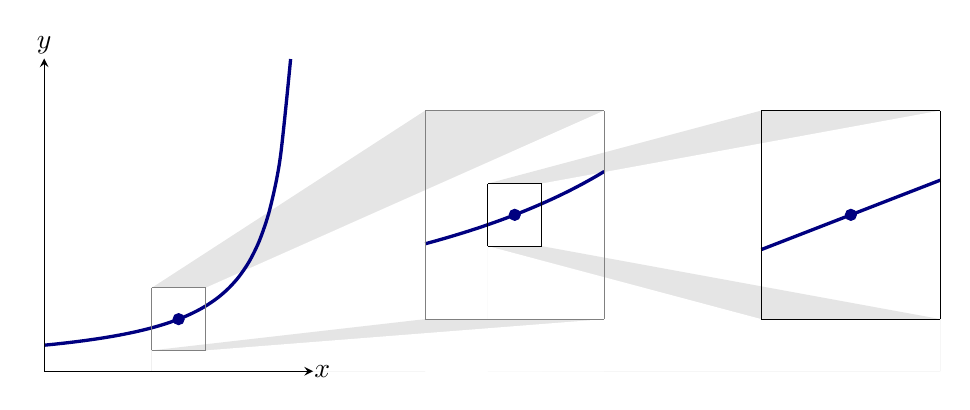
\begin{tikzpicture}
  \begin{axis}[
            domain=0:6, range=0:7,
            ymin=-.2,ymax=7,
            width=6in,
            height=2.5in, %% Hard coded height! Moreover this effects the aspect ratio of the zoom--sort of BAD
            axis lines=none,
          ]   
          \addplot [draw=none, fill=textColor!10!background] plot coordinates {(.8,1.6) (2.834,5)} \closedcycle; %% zoom fill
          \addplot [draw=none, fill=textColor!10!background] plot coordinates {(2.834,5) (4.166,5)} \closedcycle; %% zoom fill
          \addplot [draw=none, fill=background] plot coordinates {(1.2,1.6) (4.166,5)} \closedcycle; %% zoom fill
          \addplot [draw=none, fill=background] plot coordinates {(.8,1.6) (1.2,1.6)} \closedcycle; %% zoom fill

          \addplot [draw=none, fill=textColor!10!background] plot coordinates {(3.3,3.6) (5.334,5)} \closedcycle; %% zoom fill
          \addplot [draw=none, fill=textColor!10!background] plot coordinates {(5.334,5) (6.666,5)} \closedcycle; %% zoom fill
          \addplot [draw=none, fill=background] plot coordinates {(3.7,3.6) (6.666,5)} \closedcycle; %% zoom fill
          \addplot [draw=none, fill=background] plot coordinates {(3.3,3.6) (3.7,3.6)} \closedcycle; %% zoom fill
          
          \addplot [draw=none, fill=textColor!10!background] plot coordinates {(3.7,2.4) (6.666,1)} \closedcycle; %% zoom fill
          \addplot [draw=none, fill=textColor!10!background] plot coordinates {(3.3,2.4) (3.7,2.4)} \closedcycle; %% zoom fill
          \addplot [draw=none, fill=background] plot coordinates {(3.3,2.4) (5.334,1)} \closedcycle; %% zoom fill          
          \addplot [draw=none, fill=background] plot coordinates {(5.334,1) (6.666,1)} \closedcycle; %% zoom fill
          

          \addplot [draw=none, fill=textColor!10!background] plot coordinates {(.8,.4) (2.834,1)} \closedcycle; %% zoom fill
          \addplot [draw=none, fill=textColor!10!background] plot coordinates {(2.834,1) (4.166,1)} \closedcycle; %% zoom fill
          \addplot [draw=none, fill=background] plot coordinates {(1.2,.4) (4.166,1)} \closedcycle; %% zoom fill
          \addplot [draw=none, fill=background] plot coordinates {(.8,.4) (1.2,.4)} \closedcycle; %% zoom fill

          \addplot[very thick,penColor, smooth,domain=(0:1.833)] {-1/(x-2)};
          \addplot[very thick,penColor, smooth,domain=(2.834:4.166)] {3.333/(2.050-.3*x)-0.333}; %% 2.5 to 4.333
          %\addplot[very thick,penColor, smooth,domain=(5.334:6.666)] {11.11/(1.540-.09*x)-8.109}; %% 5 to 6.833
          \addplot[very thick,penColor, smooth,domain=(5.334:6.666)] {x-3}; %% 5 to 6.833
          
          \addplot[color=penColor,fill=penColor,only marks,mark=*] coordinates{(1,1)};  %% point to be zoomed
          \addplot[color=penColor,fill=penColor,only marks,mark=*] coordinates{(3.5,3)};  %% zoomed pt 1
          \addplot[color=penColor,fill=penColor,only marks,mark=*] coordinates{(6,3)};  %% zoomed pt 2

          \addplot [->,textColor] plot coordinates {(0,0) (0,6)}; %% axis
          \addplot [->,textColor] plot coordinates {(0,0) (2,0)}; %% axis
          
          \addplot [textColor!50!background] plot coordinates {(.8,.4) (.8,1.6)}; %% box around pt
          \addplot [textColor!50!background] plot coordinates {(1.2,.4) (1.2,1.6)}; %% box around pt
          \addplot [textColor!50!background] plot coordinates {(.8,1.6) (1.2,1.6)}; %% box around pt
          \addplot [textColor!50!background] plot coordinates {(.8,.4) (1.2,.4)}; %% box around pt
          
          \addplot [textColor!50!background] plot coordinates {(2.834,1) (2.834,5)}; %% zoomed box 1
          \addplot [textColor!50!background] plot coordinates {(4.166,1) (4.166,5)}; %% zoomed box 1
          \addplot [textColor!50!background] plot coordinates {(2.834,1) (4.166,1)}; %% zoomed box 1
          \addplot [textColor!50!background] plot coordinates {(2.834,5) (4.166,5)}; %% zoomed box 1

          \addplot [textColor] plot coordinates {(3.3,2.4) (3.3,3.6)}; %% box around zoomed pt
          \addplot [textColor] plot coordinates {(3.7,2.4) (3.7,3.6)}; %% box around zoomed pt
          \addplot [textColor] plot coordinates {(3.3,3.6) (3.7,3.6)}; %% box around zoomed pt
          \addplot [textColor] plot coordinates {(3.3,2.4) (3.7,2.4)}; %% box around zoomed pt

          \addplot [textColor] plot coordinates {(5.334,1) (5.334,5)}; %% zoomed box 2
          \addplot [textColor] plot coordinates {(6.666,1) (6.666,5)}; %% zoomed box 2
          \addplot [textColor] plot coordinates {(5.334,1) (6.666,1)}; %% zoomed box 2
          \addplot [textColor] plot coordinates {(5.334,5) (6.666,5)}; %% zoomed box 2

          \node at (axis cs:2.2,0) [anchor=east] {$x$};
          \node at (axis cs:0,6.6) [anchor=north] {$y$};
        \end{axis}
\end{tikzpicture}
%% \caption{Given a function $f$, if one can ``zoom in'' at $(a, f(a))$
%% sufficiently so that the graph seems to be a straight line,
%% then that line is the \textbf{tangent line} to $f$ at the point
%% determined by $(a, f(a))$.}
%% \label{figure:informal-tangent}
\end{image}
%% \todo{This image should be interactive.}

\end{comment}

More precisely, the average rate of change of a function $f$ is given by
\[
{\text{average rate of change of  $f$ }}
=\frac{f(x)-f(a)}{x-a},
\]
as the input changes from $a$ to $x$.
\begin{comment}
\begin{image}
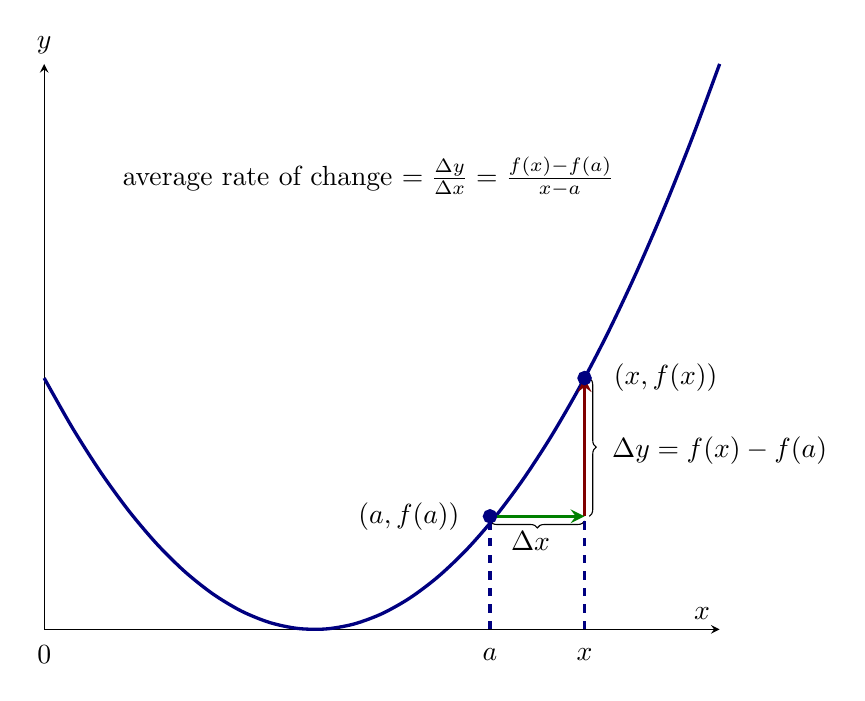
\begin{tikzpicture}
	
          \begin{axis}[
            clip=false, domain=0:2.5, axis lines =middle, xlabel=$x$,
            ylabel=$y$, every axis y label/.style={at=(current
              axis.above origin),anchor=south}, 
             width=4in,
          ticks=none ]   
                             \addplot [very thick, penColor,smooth] {(x-1)^2 };
      
       \addplot[decoration={brace,mirror,raise=.06cm},decorate,thin] plot coordinates
                       {(2,0.45) (2,1)};
                         \addplot[decoration={brace,mirror,raise=.06cm},decorate,thin] plot coordinates
                       {(1.65,0.45) (2,0.45)};
           \node at (axis cs:0,-0.1) {$0$};
             \addplot [very thick,penColor2,->]  plot coordinates {(2,0.45) (2,1)};
             \addplot [very thick,penColor4,->]  plot coordinates {(1.65,0.45) (2,0.45)};
              \addplot [very thick,penColor, dashed]  plot coordinates {(1.65,0) (1.65,0.45)};
               \addplot[only marks,very thick,penColor,mark=*]
	        coordinates{(1.65,0.45)};
	        \addplot[only marks,very thick,penColor,mark=*]
	        coordinates{(2,1)};
              % \addplot [very thick,penColor2]  plot coordinates {(1,16) (1,24)};
              \addplot [very thick,penColor, dashed]  plot coordinates {(2,0) (2,0.45)};
               \node at (axis cs:1.8,0.35) {$\Delta x$ };
    
                \node at (axis cs:2.5,0.71) {$\Delta y=f(x)-f(a)$ };
               \node at (axis cs:1.65,-0.1) {$a$ };
                \node at (axis cs:1.2,1.8) {average rate of change $=\frac{\Delta y}{\Delta x}=\frac{f(x)-f(a)}{x-a}$ };
               \node at (axis cs:2,-0.1) {$x$ };
                 \node at (axis cs:2.3,1) {$(x,f(x))$ };
                  \node at (axis cs:1.35,0.45) {$(a,f(a))$ };
        \end{axis}
\end{tikzpicture}
\end{image}
\end{comment}
 \begin{image}
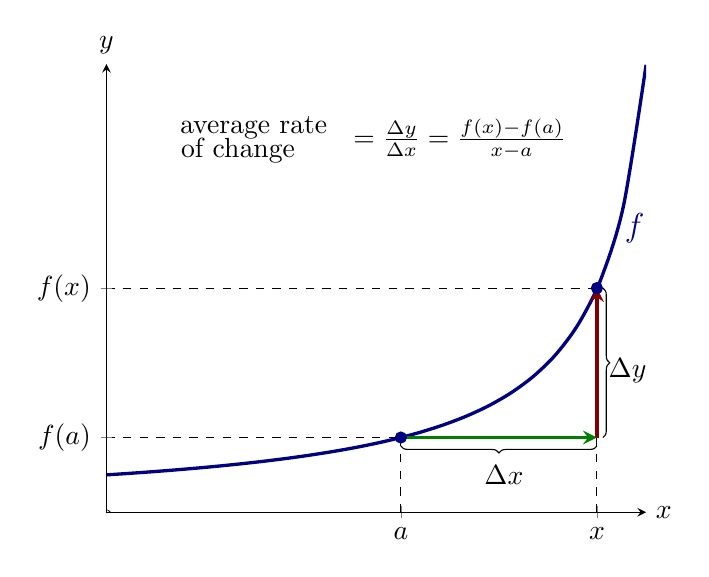
\begin{tikzpicture}
  \begin{axis}[
      domain=0:3, range=0:6,ymax=6,ymin=0,
      axis lines =left, xlabel=$x$, ylabel=$y$,
      every axis y label/.style={at=(current axis.above origin),anchor=south},
      every axis x label/.style={at=(current axis.right of origin),anchor=west},
            xtick={1,1.666}, ytick={1,3},
            xticklabels={$a$,$x$}, yticklabels={$f(a)$,$f(x)$},
            axis on top,
    ]         
         % \addplot [penColor2!15!background, domain=(0:2)] {-3.348+4.348*x};
        %  \addplot [penColor2!32!background, domain=(0:2)] {-2.704+3.704*x};
        %  \addplot [very thick,penColor2, domain=(0:2)] {-1.994+2.994*x};         
        %  \addplot [penColor2!66!background, domain=(0:2)] {-1.326+2.326*x}; 
         % \addplot [penColor2!83!background, domain=(0:2)] {-0.666+1.666*x};
	  \addplot [textColor,dashed] plot coordinates {(1,0) (1,1)};
          \addplot [textColor,dashed] plot coordinates {(0,1) (1,1)};
          \addplot [textColor,dashed] plot coordinates {(0,3) (1.666,3)};
          \addplot [textColor,dashed] plot coordinates {(1.666,0) (1.666,3)};
          \addplot [very thick,penColor, smooth,domain=(0:1.833)] {-1/(x-2)};
            \addplot[decoration={brace,mirror,raise=.06cm},decorate,thin] plot coordinates
                       {(1,0.95) (1.666,0.95)};
                         \addplot[decoration={brace,mirror,raise=.06cm},decorate,thin] plot coordinates
                       {(1.67,1) (1.67,3)};

          \addplot[color=penColor,fill=penColor,only marks,mark=*] coordinates{(1.666,3)};  %% closed hole          
          \addplot[color=penColor,fill=penColor,only marks,mark=*] coordinates{(1,1)};  %% closed hole          
         % \addplot [very thick,penColor2, smooth,domain=(0:2)] {x};
          \addplot [very thick,penColor2,->]  plot coordinates {(1.666,1) (1.666,3)};
             \addplot [very thick,penColor4,->]  plot coordinates {(1,1) (1.666,1)};
              \node at (axis cs:0,-0.1) {$0$};
               \node at (axis cs:1.35,0.5) {$\Delta x$ };
    
                \node at (axis cs:1.77,1.9) {$\Delta y$ };
                      \node at (axis cs:1.2,5) {$=\frac{\Delta y}{\Delta x}=\frac{f(x)-f(a)}{x-a}$ };
                       \node at (axis cs:0.5,5.15) {average rate};
                       \node at (axis cs:0.447,4.84){of change};
                        \node[color=penColor] at (axis cs:1.794,3.8){\large$f$};
        \end{axis}
\end{tikzpicture}
\end{image}

What happens if we compute the average rate of change of $f$  for each value of $x$ as $x$ gets closer and closer to $a$? In other words, what is the meaning of the limit
\[
     \lim_{x\to a} \frac{f(x)-f(a)}{x-a},
    \] 
    provided that the limit exists?
    
Naturally, we call this limit the \textbf{instantaneous rate of change} of the function $f$ at $a$.
%The \textit{derivative} of a function $f$ at $a$, is the instantaneous
%rate of change, and hence is the slope of the tangent line at $(a,f(a))$. 
\begin{example}
(In this example we will use abreviation AvRCh for the average rate of change,  and InRCh for the instantaneous rate of change.)

Let $f(x)=2x^2+3$.
\begin{enumerate}
\item Find the expression for the average rate of change of $f$ between the points  $a=2$ and $x=-1$.
\[
AvRCh=\frac{f(-1)-f(2)}{-1-\left(\answer[given]{2}\right)}
\]
  Now evaluate the function,
  \[
AvRCh=\frac{2(-1)^2+3-(2(2)^2+3)}{-1-\left(\answer[given]{2}\right)}.
\]
Simplify,
 \[
AvRCh=\frac{5-11}{-3}=2.
\]
\item Find  the average rate of change of $f$ between the points $a=2$ and $x$, $x\ne 2$.
\[
AvRCh=\frac{f(x)-f(2)}{x-\answer[given]{2}}
\]
 Now substitute in for the function,
\[
AvRCh=\frac{2x^2+3-11}{x-\answer[given]{2}}
\]
Simplify the top,
\[
AvRCh=\frac{2x^2-8}{x-\answer[given]{2}}.
\]
Factor,
\[
AvRCh=\frac{2(x^2-4)}{x-2}
\]
Factor and cancel,
\[
AvRCh=\frac{2(x+2)\cancel{(x-2)}}{\cancel{x-2}}=2(x+2)
\]
\item Find the instantaneous rate of change of $f$ at the point $x=2$.
\[
InRCh= \lim_{x\to 2} \frac{f(x)-f(2)}{x-2}
\]
So, the instantaneous rate of change is the limit, as $x\to 2$, of average rates of change of $f$ between points $a=2$ and $x$, for $x\ne2$. 

We have already computed an expression for the average rate of change for all $x\ne2$. 
Therefore,
\[
InRCh=\lim_{x\to 2}2(x+2)=8
\]

\end{enumerate}
\end{example}
We can arrive at the same limit,
\[
     \lim_{x\to a} \frac{f(x)-f(a)}{x-a},
    \] 

 within a completely different context.

 Have a look at the figure below.
The figure depicts a graph of the function $f$, two points on the graph, $(a,f(a))$ and $(x,f(x))$, and a \textbf{secant line} that passes  through these two points.
\begin{comment}
\begin{image}
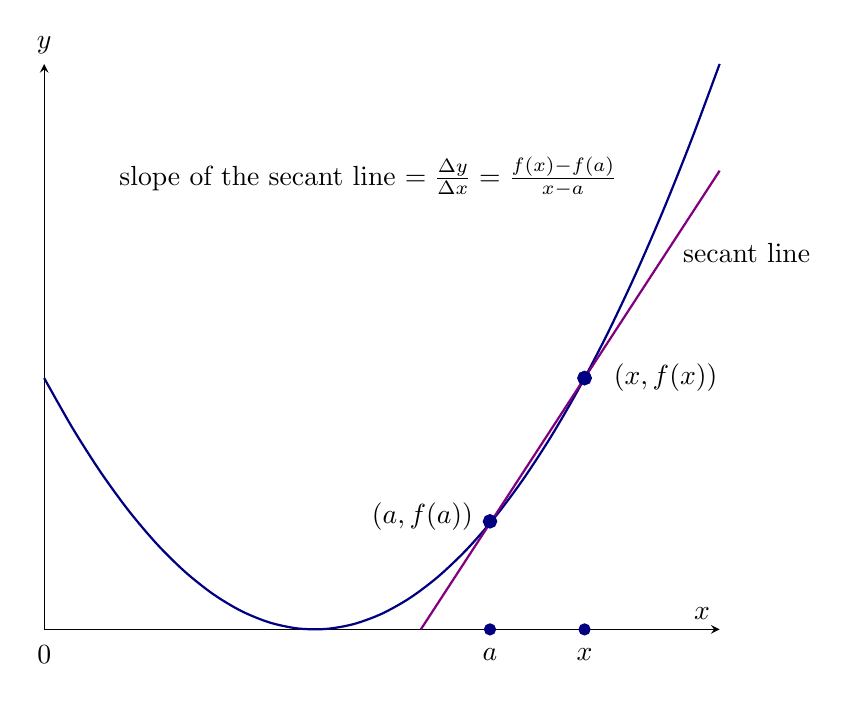
\begin{tikzpicture}
          \begin{axis}[
            clip=false, domain=0:2.5, axis lines =middle, xlabel=$x$,
            ylabel=$y$, every axis y label/.style={at=(current
              axis.above origin),anchor=south}, 
             width=4in,
          ticks=none ]   
                             \addplot [thick, penColor,smooth] {(x-1)^2 };
      
     
                     
           \node at (axis cs:0,-0.1) {$0$};
        
           
               \addplot[only marks,very thick,penColor,mark=*]
	        coordinates{(1.65,0.43)};
	        \addplot[only marks,very thick,penColor,mark=*]
	        coordinates{(2,1)};
              % \addplot [very thick,penColor2]  plot coordinates {(1,16) (1,24)};
            
                \addplot [ thick,penColor3]  plot coordinates {(1.394,0) (2.5,1.825)};
           
	        \addplot[only marks,very thick,penColor,mark=*]
	        coordinates{(2,1)};
               
      \addplot[only marks,penColor,mark=*]
	        coordinates{(2,0)};
            \addplot[only marks,penColor,mark=*]
	        coordinates{(1.65,0)};

               \node at (axis cs:1.65,-0.1) {$a$ };
                \node at (axis cs:1.2,1.8) {slope of the secant line $=\frac{\Delta y}{\Delta x}=\frac{f(x)-f(a)}{x-a}$ };
               \node at (axis cs:2,-0.1) {$x$ };
                 \node at (axis cs:2.3,1) {$(x,f(x))$ };
                  \node at (axis cs:1.4,0.45) {$(a,f(a))$ };
                   \node at (axis cs:2.6,1.5) { secant line  };
        \end{axis}
\end{tikzpicture}
\end{image}
\end{comment}
\begin{image}
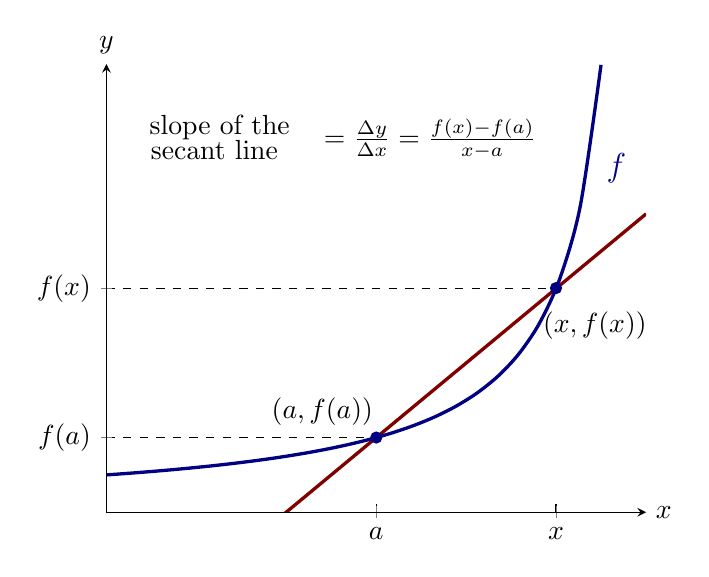
\begin{tikzpicture}
  \begin{axis}[
      domain=0:2, range=0:6,ymax=6,ymin=0,
      axis lines =left, xlabel=$x$, ylabel=$y$,
      every axis y label/.style={at=(current axis.above origin),anchor=south},
      every axis x label/.style={at=(current axis.right of origin),anchor=west},
            xtick={1,1.666}, ytick={1,3},
            xticklabels={$a$,$x$}, yticklabels={$f(a)$,$f(x)$},
            axis on top,
    ]         
         % \addplot [penColor2!15!background, domain=(0:2)] {-3.348+4.348*x};
        %  \addplot [penColor2!32!background, domain=(0:2)] {-2.704+3.704*x};
          \addplot [very thick,penColor2, domain=(0:2)] {-1.994+2.994*x};         
        %  \addplot [penColor2!66!background, domain=(0:2)] {-1.326+2.326*x}; 
         % \addplot [penColor2!83!background, domain=(0:2)] {-0.666+1.666*x};
	  \addplot [textColor,dashed] plot coordinates {(1,0) (1,0.2)};
          \addplot [textColor,dashed] plot coordinates {(0,1) (1,1)};
          \addplot [textColor,dashed] plot coordinates {(0,3) (1.666,3)};
          \addplot [textColor,dashed] plot coordinates {(1.666,0) (1.666,0.2)};
          \addplot [very thick,penColor, smooth,domain=(0:1.833)] {-1/(x-2)};
          \addplot[color=penColor,fill=penColor,only marks,mark=*] coordinates{(1.666,3)};  %% closed hole          
          \addplot[color=penColor,fill=penColor,only marks,mark=*] coordinates{(1,1)};  %% closed hole          
         % \addplot [very thick,penColor2, smooth,domain=(0:2)] {x};
        %  \addplot [very thick,penColor2,->]  plot coordinates {(1.666,1) (1.666,3)};
            % \addplot [very thick,penColor4,->]  plot coordinates {(1,1) (1.666,1)};
               \node at (axis cs:0.4,4.85) { secant line};
                 \node at (axis cs:0.42,5.15) {slope of the};
              \node at (axis cs:1.2,5) {$=\frac{\Delta y}{\Delta x}=\frac{f(x)-f(a)}{x-a}$ };
                \node at (axis cs:0.8,1.35) { $(a,f(a))$};
                  \node at (axis cs:1.81,2.5) { $(x,f(x))$};
                   \node[color=penColor] at (axis cs:1.89,4.6){\large$f$};
        \end{axis}
\end{tikzpicture}
\end{image}
The slope of this secant line is equal to $\frac{f(x)-f(a)}{x-a}$! 

This is exactly the expression for the average rate of change of $f$ as the input changes from $a$ to $x$!

Therefore,

\[
{\text{slope of secant line $=$}}{\text{ average rate of change.}}
\]
As before, we can ask ourselves: What happens as $x$ gets closer and closer to $a$?
 In other words,
   what is the meaning of the limit of slopes of secant lines through the points $(a,f(a))$ and $(x,f(x))$ as $x$ gets closer and closer to $a$?
   
    How can we interpret the limit  
    \[
     \lim_{x\to a} \frac{f(x)-f(a)}{x-a},
    \] 
    provided that the limit exists?
    
    This scenario is illustrated in the figure below. What happens as $x\to a$?
    \begin{image}
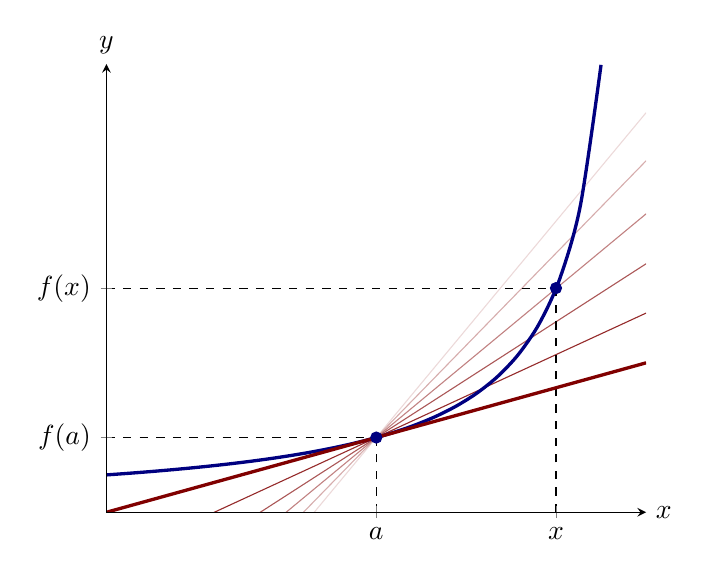
\begin{tikzpicture}
  \begin{axis}[
      domain=0:2, range=0:6,ymax=6,ymin=0,
      axis lines =left, xlabel=$x$, ylabel=$y$,
      every axis y label/.style={at=(current axis.above origin),anchor=south},
      every axis x label/.style={at=(current axis.right of origin),anchor=west},
            xtick={1,1.666}, ytick={1,3},
            xticklabels={$a$,$x$}, yticklabels={$f(a)$,$f(x)$},
            axis on top,
    ]         
          \addplot [penColor2!15!background, domain=(0:2)] {-3.348+4.348*x};
          \addplot [penColor2!32!background, domain=(0:2)] {-2.704+3.704*x};
          \addplot [penColor2!49!background, domain=(0:2)] {-1.994+2.994*x};         
          \addplot [penColor2!66!background, domain=(0:2)] {-1.326+2.326*x}; 
          \addplot [penColor2!83!background, domain=(0:2)] {-0.666+1.666*x};
	  \addplot [textColor,dashed] plot coordinates {(1,0) (1,1)};
          \addplot [textColor,dashed] plot coordinates {(0,1) (1,1)};
          \addplot [textColor,dashed] plot coordinates {(0,3) (1.666,3)};
          \addplot [textColor,dashed] plot coordinates {(1.666,0) (1.666,3)};
          \addplot [very thick,penColor, smooth,domain=(0:1.833)] {-1/(x-2)};
          \addplot[color=penColor,fill=penColor,only marks,mark=*] coordinates{(1.666,3)};  %% closed hole          
          \addplot[color=penColor,fill=penColor,only marks,mark=*] coordinates{(1,1)};  %% closed hole          
          \addplot [very thick,penColor2, smooth,domain=(0:2)] {x};
        \end{axis}
\end{tikzpicture}
\end{image}
Notice that all the secant lines in the figure pass through the given point $(a,f(a))$. What distinguishes these lines are their slopes; the slope of each line is determined by an additional point on the line, $(x,f(x))$. 
The figure suggests that``the limit of slopes of secant lines" is the slope of a special line, called the \textbf{tangent line} to the curve $y=f(x)$ at the point $(a,f(a))$.
 Notice how the tangent line and the curve are indistinguishable near the point $(a,f(a))$. If one can ``zoom in''
on the graph at $(a, f(a))$ sufficiently so that it appears to be a straight line,
then that line is the \dfn{tangent line} to $f(x)$ at the point $(a,f(a))$. This is illustrated in the figure below.
\begin{image}
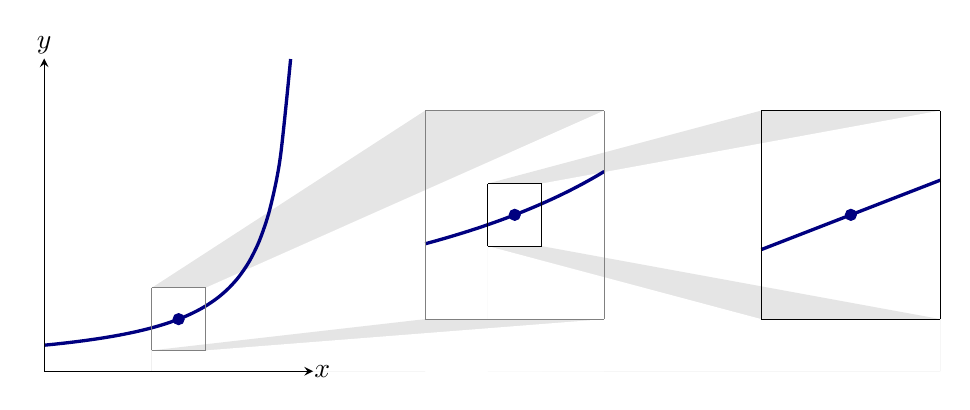
\begin{tikzpicture}
  \begin{axis}[
            domain=0:6, range=0:7,
            ymin=-.2,ymax=7,
            width=6in,
            height=2.5in, %% Hard coded height! Moreover this effects the aspect ratio of the zoom--sort of BAD
            axis lines=none,
          ]   
          \addplot [draw=none, fill=textColor!10!background] plot coordinates {(.8,1.6) (2.834,5)} \closedcycle; %% zoom fill
          \addplot [draw=none, fill=textColor!10!background] plot coordinates {(2.834,5) (4.166,5)} \closedcycle; %% zoom fill
          \addplot [draw=none, fill=background] plot coordinates {(1.2,1.6) (4.166,5)} \closedcycle; %% zoom fill
          \addplot [draw=none, fill=background] plot coordinates {(.8,1.6) (1.2,1.6)} \closedcycle; %% zoom fill

          \addplot [draw=none, fill=textColor!10!background] plot coordinates {(3.3,3.6) (5.334,5)} \closedcycle; %% zoom fill
          \addplot [draw=none, fill=textColor!10!background] plot coordinates {(5.334,5) (6.666,5)} \closedcycle; %% zoom fill
          \addplot [draw=none, fill=background] plot coordinates {(3.7,3.6) (6.666,5)} \closedcycle; %% zoom fill
          \addplot [draw=none, fill=background] plot coordinates {(3.3,3.6) (3.7,3.6)} \closedcycle; %% zoom fill
          
          \addplot [draw=none, fill=textColor!10!background] plot coordinates {(3.7,2.4) (6.666,1)} \closedcycle; %% zoom fill
          \addplot [draw=none, fill=textColor!10!background] plot coordinates {(3.3,2.4) (3.7,2.4)} \closedcycle; %% zoom fill
          \addplot [draw=none, fill=background] plot coordinates {(3.3,2.4) (5.334,1)} \closedcycle; %% zoom fill          
          \addplot [draw=none, fill=background] plot coordinates {(5.334,1) (6.666,1)} \closedcycle; %% zoom fill
          

          \addplot [draw=none, fill=textColor!10!background] plot coordinates {(.8,.4) (2.834,1)} \closedcycle; %% zoom fill
          \addplot [draw=none, fill=textColor!10!background] plot coordinates {(2.834,1) (4.166,1)} \closedcycle; %% zoom fill
          \addplot [draw=none, fill=background] plot coordinates {(1.2,.4) (4.166,1)} \closedcycle; %% zoom fill
          \addplot [draw=none, fill=background] plot coordinates {(.8,.4) (1.2,.4)} \closedcycle; %% zoom fill

          \addplot[very thick,penColor, smooth,domain=(0:1.833)] {-1/(x-2)};
          \addplot[very thick,penColor, smooth,domain=(2.834:4.166)] {3.333/(2.050-.3*x)-0.333}; %% 2.5 to 4.333
          %\addplot[very thick,penColor, smooth,domain=(5.334:6.666)] {11.11/(1.540-.09*x)-8.109}; %% 5 to 6.833
          \addplot[very thick,penColor, smooth,domain=(5.334:6.666)] {x-3}; %% 5 to 6.833
          
          \addplot[color=penColor,fill=penColor,only marks,mark=*] coordinates{(1,1)};  %% point to be zoomed
          \addplot[color=penColor,fill=penColor,only marks,mark=*] coordinates{(3.5,3)};  %% zoomed pt 1
          \addplot[color=penColor,fill=penColor,only marks,mark=*] coordinates{(6,3)};  %% zoomed pt 2

          \addplot [->,textColor] plot coordinates {(0,0) (0,6)}; %% axis
          \addplot [->,textColor] plot coordinates {(0,0) (2,0)}; %% axis
          
          \addplot [textColor!50!background] plot coordinates {(.8,.4) (.8,1.6)}; %% box around pt
          \addplot [textColor!50!background] plot coordinates {(1.2,.4) (1.2,1.6)}; %% box around pt
          \addplot [textColor!50!background] plot coordinates {(.8,1.6) (1.2,1.6)}; %% box around pt
          \addplot [textColor!50!background] plot coordinates {(.8,.4) (1.2,.4)}; %% box around pt
          
          \addplot [textColor!50!background] plot coordinates {(2.834,1) (2.834,5)}; %% zoomed box 1
          \addplot [textColor!50!background] plot coordinates {(4.166,1) (4.166,5)}; %% zoomed box 1
          \addplot [textColor!50!background] plot coordinates {(2.834,1) (4.166,1)}; %% zoomed box 1
          \addplot [textColor!50!background] plot coordinates {(2.834,5) (4.166,5)}; %% zoomed box 1

          \addplot [textColor] plot coordinates {(3.3,2.4) (3.3,3.6)}; %% box around zoomed pt
          \addplot [textColor] plot coordinates {(3.7,2.4) (3.7,3.6)}; %% box around zoomed pt
          \addplot [textColor] plot coordinates {(3.3,3.6) (3.7,3.6)}; %% box around zoomed pt
          \addplot [textColor] plot coordinates {(3.3,2.4) (3.7,2.4)}; %% box around zoomed pt

          \addplot [textColor] plot coordinates {(5.334,1) (5.334,5)}; %% zoomed box 2
          \addplot [textColor] plot coordinates {(6.666,1) (6.666,5)}; %% zoomed box 2
          \addplot [textColor] plot coordinates {(5.334,1) (6.666,1)}; %% zoomed box 2
          \addplot [textColor] plot coordinates {(5.334,5) (6.666,5)}; %% zoomed box 2

          \node at (axis cs:2.2,0) [anchor=east] {$x$};
          \node at (axis cs:0,6.6) [anchor=north] {$y$};
        \end{axis}
\end{tikzpicture}
%% \caption{Given a function $f$, if one can ``zoom in'' at $(a, f(a))$
%% sufficiently so that the graph seems to be a straight line,
%% then that line is the \textbf{tangent line} to $f$ at the point
%% determined by $(a, f(a))$.}
%% \label{figure:informal-tangent}
\end{image}
\begin{question}
Each of the following four figures depicts the graph of the same function $f$ and a line that passes through the point $(1,f(1))$.
 \begin{image}
    \begin{tabular}{cc}
      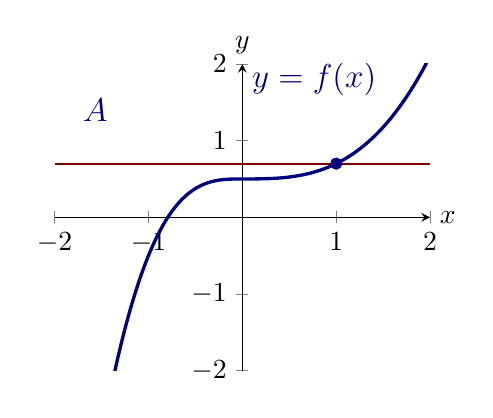
\begin{tikzpicture}
        \begin{axis}[
          domain=-2:2,
          xmin=-2, xmax=2,
          ymin=-2, ymax=2,
          width=2.5in,
          axis lines =middle, xlabel=$x$, ylabel=$y$,
          every axis y label/.style={at=(current axis.above origin),anchor=south},
          every axis x label/.style={at=(current axis.right of origin),anchor=west},
          ]
	  \addplot [very thick, penColor, smooth,domain=(-2:0)] {x^3+0.5};
	   \addplot [very thick, penColor, smooth,domain=(0:2)] {0.2*x^3+0.5};
	   \addplot[color=penColor,fill=penColor,only marks,mark=*] coordinates{(1,0.7)}; 
	      \addplot [thick,penColor2, domain=(-2:2)] {0.7};
          \node at (axis cs:-1.8, 1.4 ) [penColor,anchor=west] {\large$A$};
           \node at (axis cs:0., 1.8 ) [penColor,anchor=west] {\large$y=f(x)$};
        \end{axis}
      \end{tikzpicture}
      &
      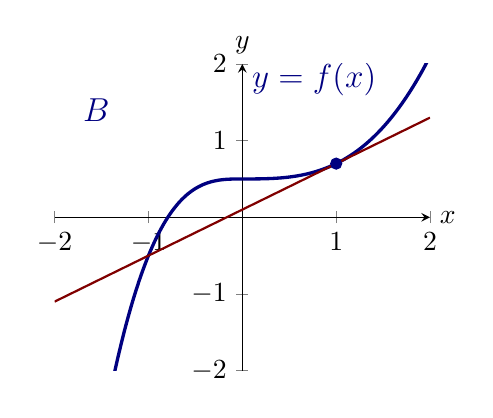
\begin{tikzpicture}
        \begin{axis}[
          domain=-2:2,
          xmin=-2, xmax=2,
          ymin=-2, ymax=2,
          width=2.5in,
          axis lines =middle, xlabel=$x$, ylabel=$y$,
          every axis y label/.style={at=(current axis.above origin),anchor=south},
          every axis x label/.style={at=(current axis.right of origin),anchor=west},
          ]
	   \addplot [very thick, penColor, smooth,domain=(-2:0)] {x^3+0.5};
	   \addplot [very thick, penColor, smooth,domain=(0:2)] {0.2*x^3+0.5};
	   \addplot [thick,penColor2, domain=(-2:2)] {0.6*x+.1};
	   \addplot[color=penColor,fill=penColor,only marks,mark=*] coordinates{(1,0.7)}; 
          \node at (axis cs:-1.8, 1.4 ) [penColor,anchor=west] {\large$B$};
           \node at (axis cs:0., 1.8 ) [penColor,anchor=west] {\large$y=f(x)$};
        \end{axis}
      \end{tikzpicture}\\
      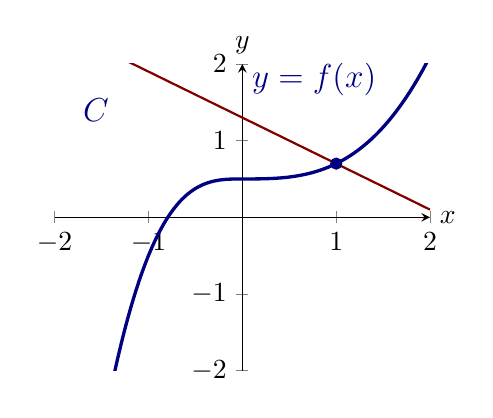
\begin{tikzpicture}
        \begin{axis}[
          domain=-2:2,
          xmin=-2, xmax=2,
          ymin=-2, ymax=2,
          width=2.5in,
          axis lines =middle, xlabel=$x$, ylabel=$y$,
          every axis y label/.style={at=(current axis.above origin),anchor=south},
          every axis x label/.style={at=(current axis.right of origin),anchor=west},
          ]
	  \addplot [very thick, penColor, smooth,domain=(-2:0)] {x^3+0.5};
	   \addplot [very thick, penColor, smooth,domain=(0:2)] {0.2*x^3+0.5};
	   \addplot [thick,penColor2, domain=(-2:2)] {-0.6*x+1.3};
	  \addplot[color=penColor,fill=penColor,only marks,mark=*] coordinates{(1,0.7)}; 
          \node at (axis cs:-1.8, 1.4 ) [penColor,anchor=west] {\large$C$};
            \node at (axis cs:0., 1.8 ) [penColor,anchor=west] {\large$y=f(x)$};
        \end{axis}
      \end{tikzpicture}
      &
      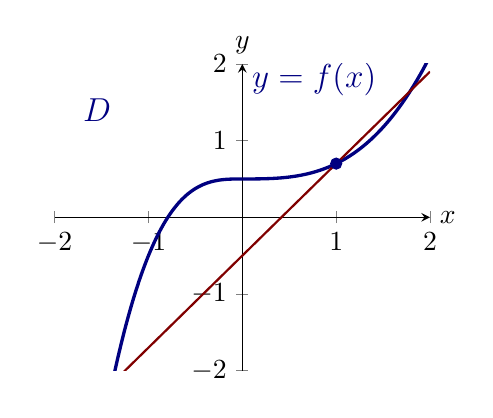
\begin{tikzpicture}
        \begin{axis}[
          domain=-2:2,
          xmin=-2, xmax=2,
          ymin=-2, ymax=2,
          width=2.5in,
          axis lines =middle, xlabel=$x$, ylabel=$y$,
          every axis y label/.style={at=(current axis.above origin),anchor=south},
          every axis x label/.style={at=(current axis.right of origin),anchor=west},
          ]
	  \addplot [very thick, penColor, smooth,domain=(-2:0)] {x^3+0.5};
	   \addplot [very thick, penColor, smooth,domain=(0:2)] {0.2*x^3+0.5};
	  \addplot[color=penColor,fill=penColor,only marks,mark=*] coordinates{(1,0.7)}; 
          \node at (axis cs:-1.8, 1.4 ) [penColor,anchor=west] {\large$D$};
            \node at (axis cs:0., 1.8 ) [penColor,anchor=west] {\large$y=f(x)$};
             \addplot [thick,penColor2, domain=(-2:2)] {1.2*x-0.5};
        \end{axis}
      \end{tikzpicture}
    \end{tabular}
  \end{image}
Only one of the figures depicts the line tangent to the curve $y=f(x)$ at the point $(1,f(1))$. Which one?
\begin{multipleChoice}
\choice { Figure A}
\choice[correct]{Figure B}
\choice {Figure C}
\choice {Figure D}
\end{multipleChoice}
\begin{explanation}
Only the line in figure $B$ looks indistinguishable from the curve $y=f(x)$ near the point $(1,f(1))$.
\end{explanation}
\end{question}
Obviously, the limit
 \[
     \lim_{x\to a} \frac{f(x)-f(a)}{x-a},
    \] 
    has many different interpretations, depending on the context, such as the slope of the tangent line, the  instantaneous rate of change, and the instantaneous velocity.
    
    Therefore, this limit deserves a special name that could be used regardless of the context.
    \begin{definition}
  The \dfn{derivative} of $f$ at $a$, denoted $f'(a)$, is given by
  \[
 f'(a) = \lim_{x\to a} \frac{f(x) - f(a)}{x-a},
  \]
 provided that the limit exists. We say that $f$ is \dfn{differentiable}
  at $a$ if  this limit exists. Otherwise,  we say that  $f$ is \dfn{non-differentiable} at $a$.
\end{definition}

The definition of the derivative allows us to define a tangent line precisely.
  \begin{definition}
  Let $f$ be a function differentiable at $a$. The \dfn{ line tangent to the curve} $y=f(x)$ at the point $(a,f(a))$ is the line that passes through the point $(a,f(a))$ whose slope is equal to $f'(a)$.
    \end{definition}
  
  Naturally, by the point-slope equation of the line, it follows that the tangent line is given by the equation
  \[
 y = f(a)+f'(a)(x-a).
  \]

      \begin{question}
            Let $f$ be a function given by $f(x) = 4x-3$.
	What is the instantaneous rate of change of $f$ at $a$, where $a$ is any real number?
	\begin{hint}
		The rate of change is given by $f'(a)$, and so is the slope of the tangent line to the curve $y=f(x)$ at the point $(a,f(a))$.
	\end{hint}
	\begin{hint}
		The line tangent to the curve $y=f(x) = 4x-3$, is simply the curve itself!
	\end{hint}
	\begin{prompt}
		The derivative is the slope of the line $y= 4x-3$! Therefore,  $f'(a)=\answer{4}$, for all real numbers $a$.
	\end{prompt}
	\begin{hint}
		 Of course, we can verify this reasoning by simply computing $f'(a)$, using the definition of the derivative.
		 \[
 f'(a) = \lim_{x\to a} \frac{f(x) - f(a)}{x-a}.
  \]
Replace $f$ with its formula,
		\[
 f'(a) = \lim_{x\to a} \frac{(4x-3)-(4a-3)}{x-a}.
  \]
		Simplify the numerator,
			\[
 f'(a) = \lim_{x\to a} \frac{4x-4a}{x-a}.
  \]

		Factor the numerator,
		\[
 f'(a) = \lim_{x\to a} \frac{4\cancel{(x-a)}}{\cancel{x-a}}.
  \]
 Compute the limit,

		\[
 f'(a) =4.
  \]

			\end{hint}
\end{question}


But, most functions are not linear, and  their graphs are not  straight lines.  Therefore, the computation of the derivative is not as simple as in the previous example.

\begin{example}
	Let $f(x) = 2x^2+3$.
	
	 Find the slope of the tangent line to the curve $y=f(x)$ at the point $(2,f(2))$.
			\begin{explanation}
			  Finding the slope of the tangent line at the point $(2,f(2))$ means finding $f'(2)$
		\[
 f'(2) = \lim_{x\to 2} \frac{f(x) - f(2)}{x-2}
  \]
But, this limit gives us the instantaneous rate of change of $f$ at $a=2$, which was computed in our first example!
Therefore,	
the slope of the tangent line is 
\[
 f'(2) = \lim_{x\to 2} \frac{f(x) - f(2)}{x-2}=8.
  \]
		 	\end{explanation}
			  \begin{onlineOnly}
  We can confirm our results by looking at the graph of $y=f(x)$ and the line $y=x-1$. 
  \begin{image}
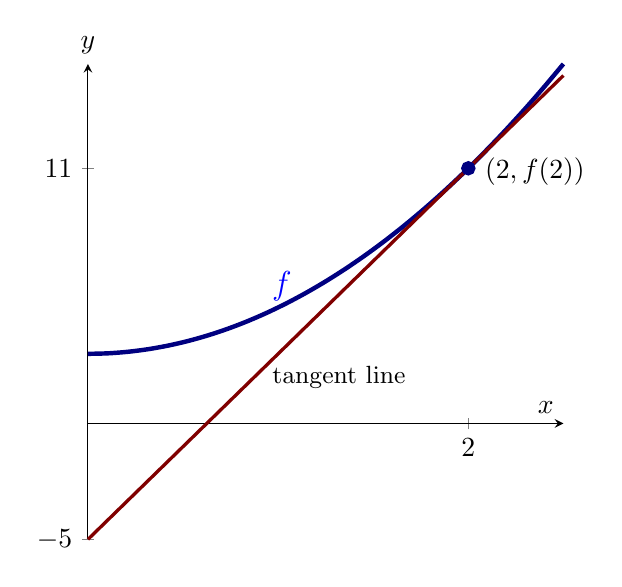
\begin{tikzpicture}
	
          \begin{axis}[
            clip=false, domain=0:2.5, axis lines =middle, xlabel=$x$,
            ylabel=$y$, every axis y label/.style={at=(current
              axis.above origin),anchor=south}, 
             width=3in,
             height=3in,
          xtick={2}, ytick={-5,11}, ]   
                             \addplot [ultra thick, penColor,smooth] {2*x^2+3 };
                                  \addplot [very thick, penColor2,smooth] {8*x-5 };
                  \addplot[only marks,very thick,penColor,mark=*]
	        coordinates{(2,11)};
              % \addplot [very thick,penColor2]  plot coordinates {(1,16) (1,24)};
              
                  \node at (axis cs:2.35,10.85) {$(2,f(2))$ };
                   \node[blue] at (axis cs:1.02,5.9) {\large$f$ };
                   \node at (axis cs:1.32,2) { \small tangent line  };
        \end{axis}
\end{tikzpicture}
\end{image}
  \end{onlineOnly}
			
	\end{example}
	\begin{example}
	Let $f(x) = \frac{1}{3-x}$.
  Find an equation for the line tangent to the curve $y=f(x)$ at the point $(2, 1)$.
  \begin{explanation}
    To find an equation for a line, we need two pieces of information.  We need to know
    a point on the line, and we need to know the slope of the line.  In this question, we are given
    that  the point $(2,1)$ is on the line.  So, we need to find the slope of the tangent line.
    Finding the slope of the tangent line at the point $(2,1)$ means finding $f'(2)$.
    
    Start by writing out the definition of the derivative,
    \[
    f'(2) = \lim_{x\to 2} \frac{f\left(\answer[given]{x}\right)-f\left(2\right)}{x-2} = \lim_{x\to 2} \frac{\frac{1}{3-x}-1}{x-2}.
    \]
    Multiply by $\frac{3-x}{3-x}$ to clear the fraction in the numerator,
    \[
    f'(2) = \lim_{x\to 2} \frac{1 - \left(\answer[given]{3-x}\right)}{(x-2)(3-x)}.
    \]
    Combine like-terms in the numerator,
    \[
    f'(2) = \lim_{x\to 2} \frac{\cancel{x-2}}{\cancel{(x-2)}(3-x)},
    \]
    	
    Take the limit as $x$ goes to $2$,
    \[
    f'(2)= \lim_{x\to 2} \frac{1}{3-x} = \answer[given]{1}.
    \]
    We are looking for an equation of the line through the point
    $(2,1)$ with slope $m = f'(2) = 1$.  The point-slope formula tells
    us that the line has equation given by
    \[
    y= 1+\answer[given]{x-2 },
    \]
    or $y=x-1$.
  \begin{onlineOnly}
  We can confirm our results by looking at the graph of $y=f(x)$ and the line $y=x-1$. 
  \begin{image}
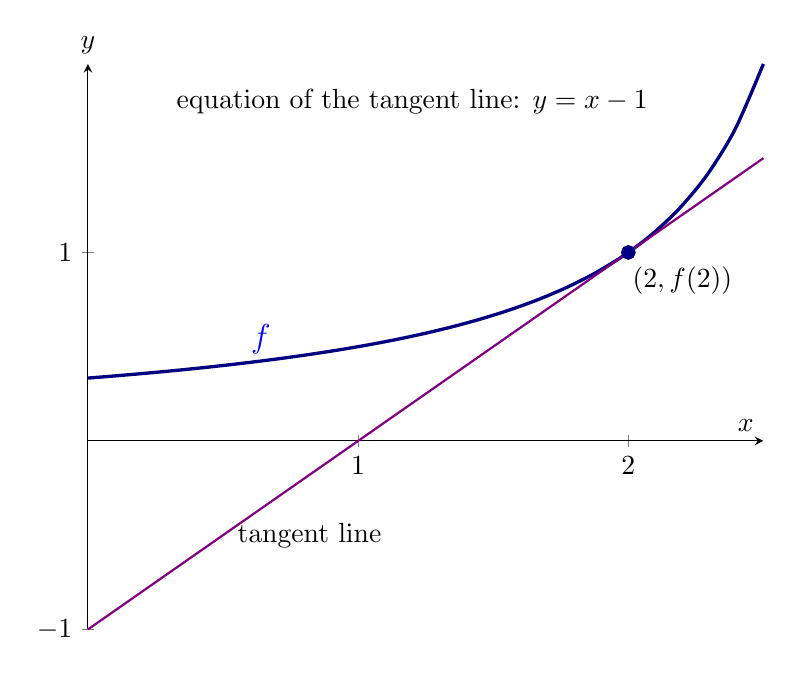
\begin{tikzpicture}
	
          \begin{axis}[
            clip=false, domain=0:2.5, axis lines =middle, xlabel=$x$,
            ylabel=$y$, every axis y label/.style={at=(current
              axis.above origin),anchor=south}, 
             width=4in,
          xtick={1,2}, ytick={-1,1,3}, ]   
                             \addplot [very thick, penColor,smooth] {1/(3-x) };
               
	        \addplot[only marks,very thick,penColor,mark=*]
	        coordinates{(2,1)};
              % \addplot [very thick,penColor2]  plot coordinates {(1,16) (1,24)};
            
                \addplot [ thick,penColor3]  plot coordinates {(0,-1) (2.5,1.5)};
           
	        \addplot[only marks,very thick,penColor,mark=*]
	        coordinates{(2,1)};
             \addplot[only marks,penColor,mark=*]
	        coordinates{(2,1)};
                       \node at (axis cs:1.2,1.8) {equation of the tangent line: $y=x-1$ };
                  \node at (axis cs:2.2,0.85) {$(2,f(2))$ };
                   \node[blue] at (axis cs:0.64,0.54) {\large$f$ };
                   \node at (axis cs:0.82,-.5) { tangent line  };
        \end{axis}
\end{tikzpicture}
\end{image}

  \end{onlineOnly}
  \end{explanation}
\end{example}
\begin{example}
  An object moving along a straight line has position given by
  $s(t) = \sqrt{t+3}$, where position is measured in meters and time in seconds.  Find the (instantaneous) velocity of the object at time $t=6$.
  \begin{explanation}
    Velocity is the instantaneous rate of change of position with respect to
    time.  We are being asked to find $v(6)=s'(6)$.  We have to adjust the
    definition of the the derivative, namely, replace $x$ with $t$,
    \[
   s'(6) = \lim_{t \to 6} \frac{s(t)-s(6)}{t-6} = \lim_{t\to 6} \frac{\sqrt{\answer[given]{t+3}}-3}{t-6}.
    \]
    Multiply by $\frac{\sqrt{t+3}+3}{\sqrt{t+3}+3}$, in order to rationalize the expression,
    \[
    s'(6) = \lim_{t\to 6} \left(\frac{\sqrt{t+3}-3}{t-6} \right)\left(\frac{\sqrt{t+3}+3}{\sqrt{t+3}+3} \right).
    \]		
    Now simplify the numerator,
    \[
    s'(6) = \lim_{t \to 6} \frac{t+3 - 9}{(t-6)\left(\sqrt{t+3}+3 \right)}.
    \]
    Combine like-terms,
    \[
   s'(6)= \lim_{t \to 6} \frac{\cancel{t-6}}{\cancel{(t-6)}\left(\sqrt{t+3}+3\right)}.
    \]
     Take the limit as $t$ goes to $6$,
    \[
    s'(6)= \lim_{t\to 6} \frac{1}{\sqrt{t+3}+3}=\answer[given]{\frac{1}{6}}.
    \]
  
   
    The object has velocity $\frac{1}{6}$ $\frac{m}{s}$ at time $t=6$.
    
	  \begin{onlineOnly}
	Below we can see the graph of $s=s(t)$ and the tangent line at $t=6$, with a slope of $\frac{1}{6}$. 
	Notice, again, how the line fits the graph of the function $s$ near the point $(6,3)$. 
		 \begin{image}
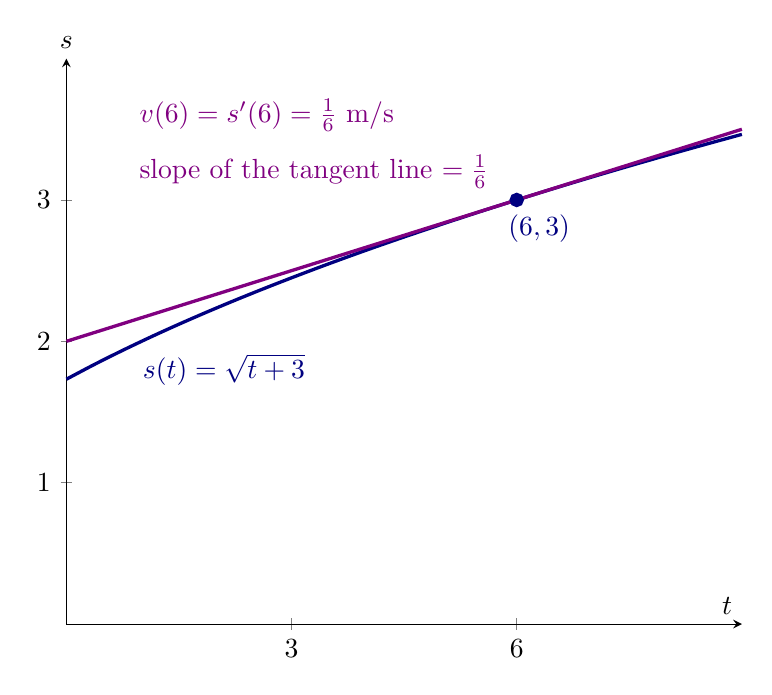
\begin{tikzpicture}
          \begin{axis}[
            clip=false, domain=0:9, range=0:9,ymax=4,ymin=0, axis lines =middle, xlabel=$t$,
            ylabel=$s$, every axis y label/.style={at=(current
              axis.above origin),anchor=south}, 
             width=4in,
          xtick={0,3,6}, ytick={1,2,3}, ]   
                             \addplot [very thick, penColor,smooth] {(x+3)^(1/2) };
              
	        \addplot[only marks,very thick,penColor,mark=*]
	        coordinates{(6,3)};
              % \addplot [very thick,penColor2]  plot coordinates {(1,16) (1,24)};
     \addplot [ very thick,penColor3]  plot coordinates {(0,2) (9,3.5)};
  \node[ thick,penColor]at (axis cs:2.1,1.8) { $s(t)=\sqrt{t+3}$ };
   \node[ thick,penColor3]at (axis cs:2.67,3.6) {$v(6)=s'(6)=\frac{1}{6}$ m/s };
                       \node[ thick,penColor3]at (axis cs:3.3,3.2) {slope of the tangent line $=\frac{1}{6}$ };
                        \node[ thick,penColor]at (axis cs:6.3,2.8) { $(6,3)$ };
        \end{axis}
\end{tikzpicture}
\end{image}
	  \end{onlineOnly}
	\end{explanation}
\end{example}

\begin{comment}
Suppose the difference between $x$ and $a$ is some small number $h$.  That
is $x-a=h$ or $x=a+h$.  Substituting this in to our definition of the derivative gives us
an alternate way of writing the definition of the derivative at the point $a$.
\[
f'(a) = \lim_{h\to 0} \frac{f(a+h)-f(a)}{(a+h)-a} = \frac{f(a+h)-f(a)}{h}.
\]
\end{comment}
\begin{comment}
\begin{example}
  If $f(x) = x^2-2x$, find the slope of the secant line through $x=2$ and $x=2+h$, in terms of $h$.
  \begin{explanation}
    Start with the slope formula we just found,
    \[
    \frac{\Delta y}{\Delta x} = \frac{f\left(\answer[given]{2+h}\right)-f\left(2\right)}{\answer[given]{h}}.
    \]
    Now substitute in for the function we know,
    \[
    \frac{\Delta y}{\Delta x} = \frac{\answer[given]{(2+h)^2-2(2+h)} -0}{h}.
    \]
    Now expand the numerator of the fraction,
    \[
    \frac{\Delta y}{\Delta x} = \frac{4+4h+h^2-4-2h }{h}.
    \]
    Now combine like-terms,
    \[
    \frac{\Delta y}{\Delta x} = \frac{2h+h^2}{h}.
    \]
    Factor an $h$ from every term in the numerator,
    \[
    \frac{\Delta y}{\Delta x} = \frac{h\left(\answer[given]{2+h}\right)}{h}.
    \]
    Cancel $h$ from the numerator and denominator,
    \[
    \frac{\Delta y}{\Delta x} = \answer[given]{2+h}. 
    \]
  \end{explanation}
\end{example}


\end{comment}
\begin{comment}
The following diagram shows the secant lines for several values of
$h$, as well as the tangent line at $(a,f(a))$.

\begin{image}
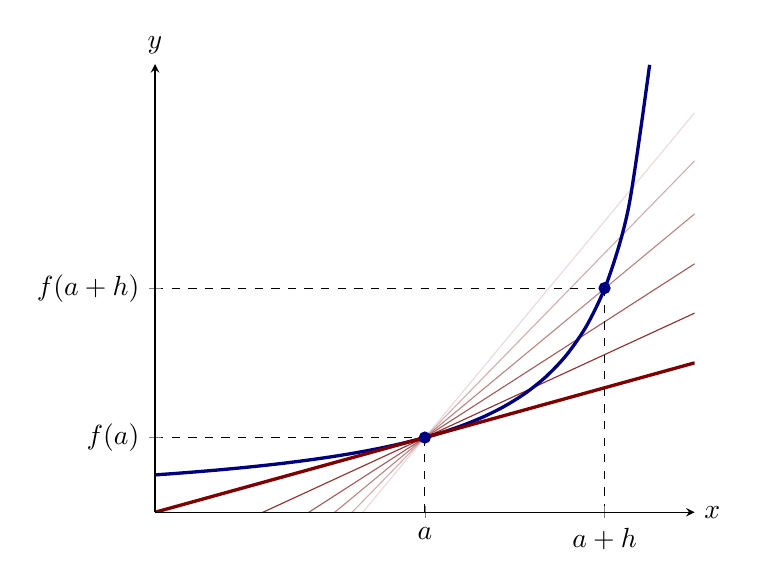
\begin{tikzpicture}
  \begin{axis}[
      domain=0:2, range=0:6,ymax=6,ymin=0,
      axis lines =left, xlabel=$x$, ylabel=$y$,
      every axis y label/.style={at=(current axis.above origin),anchor=south},
      every axis x label/.style={at=(current axis.right of origin),anchor=west},
            xtick={1,1.666}, ytick={1,3},
            xticklabels={$a$,$a+h$}, yticklabels={$f(a)$,$f(a+h)$},
            axis on top,
    ]         
          \addplot [penColor2!15!background, domain=(0:2)] {-3.348+4.348*x};
          \addplot [penColor2!32!background, domain=(0:2)] {-2.704+3.704*x};
          \addplot [penColor2!49!background, domain=(0:2)] {-1.994+2.994*x};         
          \addplot [penColor2!66!background, domain=(0:2)] {-1.326+2.326*x}; 
          \addplot [penColor2!83!background, domain=(0:2)] {-0.666+1.666*x};
	  \addplot [textColor,dashed] plot coordinates {(1,0) (1,1)};
          \addplot [textColor,dashed] plot coordinates {(0,1) (1,1)};
          \addplot [textColor,dashed] plot coordinates {(0,3) (1.666,3)};
          \addplot [textColor,dashed] plot coordinates {(1.666,0) (1.666,3)};
          \addplot [very thick,penColor, smooth,domain=(0:1.833)] {-1/(x-2)};
          \addplot[color=penColor,fill=penColor,only marks,mark=*] coordinates{(1.666,3)};  %% closed hole          
          \addplot[color=penColor,fill=penColor,only marks,mark=*] coordinates{(1,1)};  %% closed hole          
          \addplot [very thick,penColor2, smooth,domain=(0:2)] {x};
        \end{axis}
\end{tikzpicture}
\end{image}
%\todo{This image should be interactive.}


Notice that as $a+h$ approaches $a$, the slopes of the secant lines are approaching
the slope of the tangent line.  This leads to the \textit{definition of the derivative}:
\end{comment}
\begin{comment}
\begin{definition}
  The \dfn{derivative} of $f$ at $a$ is 
  \[
  \eval{\ddx f(x)}_{x=a} = \lim_{h\to 0} \frac{f(a+h) - f(a)}{h}.
  \]
  If this limit exists, then we say that $f$ is \dfn{differentiable}
  at $a$.  If this limit does not exist for a given value of $a$, then
  $f$ is \dfn{non-differentiable} at $a$.
\end{definition}

\end{comment}
\begin{comment}

\begin{question} 
    Which of the following computes the derivative, $\eval{\ddx f(x)}_{x=a}$?
    \begin{selectAll}
      \choice{$\lim_{h\to 0}\frac{(f(a)+h) - f(a)}{(a+h)-a}$}
      \choice[correct]{$\lim_{h\to 0}\frac{f(a+h) - f(a)}{(a+h)-a}$}
      \choice{$\lim_{h\to 0}\frac{(f(a)-h) - f(a)}{(a-h)-a}$}
      \choice[correct]{$\lim_{h\to 0}\frac{f(a-h) - f(a)}{(a-h)-a}$}
      \choice{$\lim_{h\to 0}\frac{f(a) - (f(a)+h)}{a-(a+h)}$}
      \choice[correct]{$\lim_{h\to 0}\frac{f(a) - f(a+h)}{a-(a+h)}$}
      \choice{$\lim_{h\to 0}\frac{f(a) - (f(a)-h)}{a-(a-h)}$}
      \choice[correct]{$\lim_{h\to 0}\frac{f(a) - f(a-h)}{a-(a-h)}$}
    \end{selectAll}
\end{question}
\end{comment}
\begin{comment}
Recalling our original characterization of the slope of the secant line
between $a$ and $x$ which is near by to $a$.  We see that we could also
calculate the derivative of a function by letting $x$ go to $a$.  This 
gives us the following definition:

\begin{definition}
	The \dfn{derivative} of $f$ at $a$ is
	\[
	\eval{\ddx f(x)}_{x=a} = \lim_{x\to a} \frac{f(x) - f(a)}{x-a}.
	\]
\end{definition}
\end{comment}
\begin{comment}

\begin{definition}\index{derivative!notation}
  There are several different notations for the derivative.  The two we'll mainly be using are
  \[
  \eval{\ddx f(x)}_{x=a} = f'(a).
  \]
\end{definition}
\end{comment}
\begin{comment}
\begin{example}
	Find the derivative of $f(x) = x^2+x+1$ at $x=-1$ using the $x\to a$
	characterization.
	\begin{explanation}
		Start with the definition of the derivative,
		\[
		f'(-1) = \lim_{x\to-1}\frac{f\left(x\right)-f\left(\answer[given]{-1}\right)}{x-(-1)}.
		\] 
		Replace $f$ with its formula,
		\[
		f'(-1) = \lim_{x\to-1}\frac{x^2+x+1 - 1}{x+1}.
		\]
		Simplify the top,
		\[
		f'(-1) = \lim_{x\to-1}\frac{x^2+x}{x+1}.
		\]
		Factor,
		\[
		f'(-1) = \lim_{x\to-1}\frac{x\left(\answer[given]{x+1}\right)}{x+1}.
		\]
		Cancel the $x+1$ in the numerator and denominator,
		\[
		f'(-1) = \lim_{x\to-1}x.
		\]
		The expression inside the limit is continuous everywhere, so
		evaluate the limit by plugging in,
		\[
		f'(-1) = \answer[given]{-1}.
		\]
	\end{explanation}
\end{example}
\end{comment}
\end{document}
